\chapter{Dynamical Systems Language}
\label{ch:dynamical-systems-language}

\textit{Clustered spiking networks can look like they are wandering among remembered states. Before deciding whether that wandering is noise-driven multistability or deterministic mesoscopic chaos, we need a precise language for states, trajectories, attractors, perturbations, and stability.}

% ============================================================
\section{Why Start With Dynamics?}
\label{sec:why-start-with-dynamics}
% ============================================================

The later chapters study networks with many neurons, many clusters, excitation, inhibition, finite-size fluctuations, and quenched heterogeneity. The raw model is high dimensional, but the central questions are dynamical:

\begin{itemize}
  \item Does the network return to a stable activity pattern after a small perturbation?
  \item Does it switch only because a finite population produces random fluctuations?
  \item Or does the macroscopic cluster activity keep moving even when finite-size noise is removed?
\end{itemize}

These are not questions about a single trace alone. A single trace can show irregular switching in both a multistable system with noise and a chaotic deterministic system. The distinction lives in the structure of the state space and in how nearby trajectories behave.

By the end of this chapter, the reader should be able to translate an activity model into a state-space picture, test local stability with a Jacobian, explain what an attractor basin means, and state why a positive Lyapunov exponent is evidence for deterministic sensitivity rather than ordinary trial-to-trial variability.

In this chapter, a ``state'' will be an abstract vector $x(t)$. Later, $x(t)$ might contain membrane voltages, filtered spike trains, population rates, or cluster activities. We first learn the language in a deterministic setting,
%
\begin{equation}
  \frac{d x}{d t} = F(x;\theta),
  \qquad x(t) \in \mathcal{X} \subseteq \mathbb{R}^d,
  \label{eq:deterministic-flow}
\end{equation}
%
where $F$ is the vector field and $\theta$ denotes parameters such as recurrent coupling strength, cluster strength, or quenched variability. The vector field assigns a velocity to every state. The state space $\mathcal{X}$ is the set of possible values of $x$: for a two-variable rate model it might be a plane, while for a network of $Q$ paired E/I clusters it might be a $2Q$-dimensional region of population activities.

Equation~\eqref{eq:deterministic-flow} is deliberately simple. It lets us define the concepts that survive in more complicated forms when stochastic spike trains and finite-size effects are added in \cref{ch:stochastic-processes-neural-dynamics}.

% ============================================================
\section{States and Trajectories}
\label{sec:states-trajectories}
% ============================================================

A \emph{trajectory} is the curve traced by $x(t)$ in state space as time advances. If the initial condition is $x(0)=x_0$, the solution is often denoted $\phi_t(x_0)$, where $\phi_t$ is the flow map:
%
\begin{equation}
  x(t) = \phi_t(x_0).
  \label{eq:flow-map}
\end{equation}
%
The notation emphasizes that the current state is obtained by applying the same dynamical rule to an initial state for time $t$.

In a clustered network, the same idea appears at several resolutions. A microscopic state could include all membrane voltages and synaptic variables. A mesoscopic state might include one filtered activity variable per population in each cluster, for example
%
\begin{equation}
  x(t) =
  \bigl(R_1^E(t),R_1^I(t),\ldots,R_Q^E(t),R_Q^I(t)\bigr),
  \label{eq:cluster-state-vector}
\end{equation}
%
where $R_a^E(t)$ and $R_a^I(t)$ are filtered excitatory and inhibitory population activities in cluster $a$. Chapter~\ref{ch:stochastic-processes-neural-dynamics} reserves $A_a^\alpha(t)$ for the raw population spike train and uses $R_a^\alpha(t)=(\epsilon*A_a^\alpha)(t)$ for the explicitly filtered continuous activity. The mesoscopic description throws away many microscopic details, but it keeps the variables needed to ask whether whole clusters are active, inactive, switching, or fluctuating chaotically.

A state-space picture is useful because it separates three ideas that are easily confused in time traces:

\begin{description}
  \item[Where the system is.] This is the current point $x(t)$.
  \item[Where the system tends to go.] This is the vector field $F(x;\theta)$.
  \item[How the system reacts to perturbations.] This is determined by the local geometry of $F$ and, globally, by the basins and attractors.
\end{description}

% ============================================================
\section{Fixed Points and Local Stability}
\label{sec:fixed-points-local-stability}
% ============================================================

A \emph{fixed point} is a state $x^\ast$ where the deterministic velocity vanishes:
%
\begin{equation}
  F(x^\ast;\theta)=0.
  \label{eq:fixed-point}
\end{equation}
%
If the system reaches $x^\ast$, it stays there. In neural terms, a fixed point might represent a stable low-rate asynchronous state, a persistent activity pattern with a particular set of active clusters, or a balanced state in which excitation and inhibition cancel on average.

The important question is not only whether $x^\ast$ exists, but whether it is stable. Perturb the state by a small vector $\delta x(t)$:
%
\begin{equation}
  x(t) = x^\ast + \delta x(t).
  \label{eq:perturbation-definition}
\end{equation}
%
Taylor expansion of the vector field gives
%
\begin{equation}
  \frac{d}{dt}\delta x(t)
  =
  J(x^\ast)\,\delta x(t)
  + \text{higher-order terms},
  \qquad
  J_{ij}(x^\ast)
  =
  \left.\frac{\partial F_i}{\partial x_j}\right|_{x=x^\ast}.
  \label{eq:linearization-jacobian}
\end{equation}
%
The matrix $J(x^\ast)$ is the \emph{Jacobian}. It is the best linear approximation to the dynamics near the fixed point. The entry $J_{ij}$ measures how the velocity of coordinate $i$ changes when coordinate $j$ is perturbed.

If $J$ has eigenvectors $v_k$ and eigenvalues $\lambda_k$, the linearized perturbation decomposes into modes
%
\begin{equation}
  \delta x(t)
  =
  \sum_k c_k e^{\lambda_k t} v_k
  \label{eq:linear-mode-decomposition}
\end{equation}
%
when $J$ is diagonalizable. The real part of $\lambda_k$ sets whether mode $k$ grows or decays. A fixed point is linearly stable when every eigenvalue has negative real part:
%
\begin{equation}
  \mathrm{Re}\,\lambda_k < 0
  \quad \text{for all } k.
  \label{eq:linear-stability-condition}
\end{equation}
%
If even one eigenvalue has positive real part, some perturbations grow. This is why the Jacobian is a diagnostic tool: it turns the geometric question ``do small perturbations return?'' into a spectral question about eigenvalues.

\begin{figure}[h]
\centering
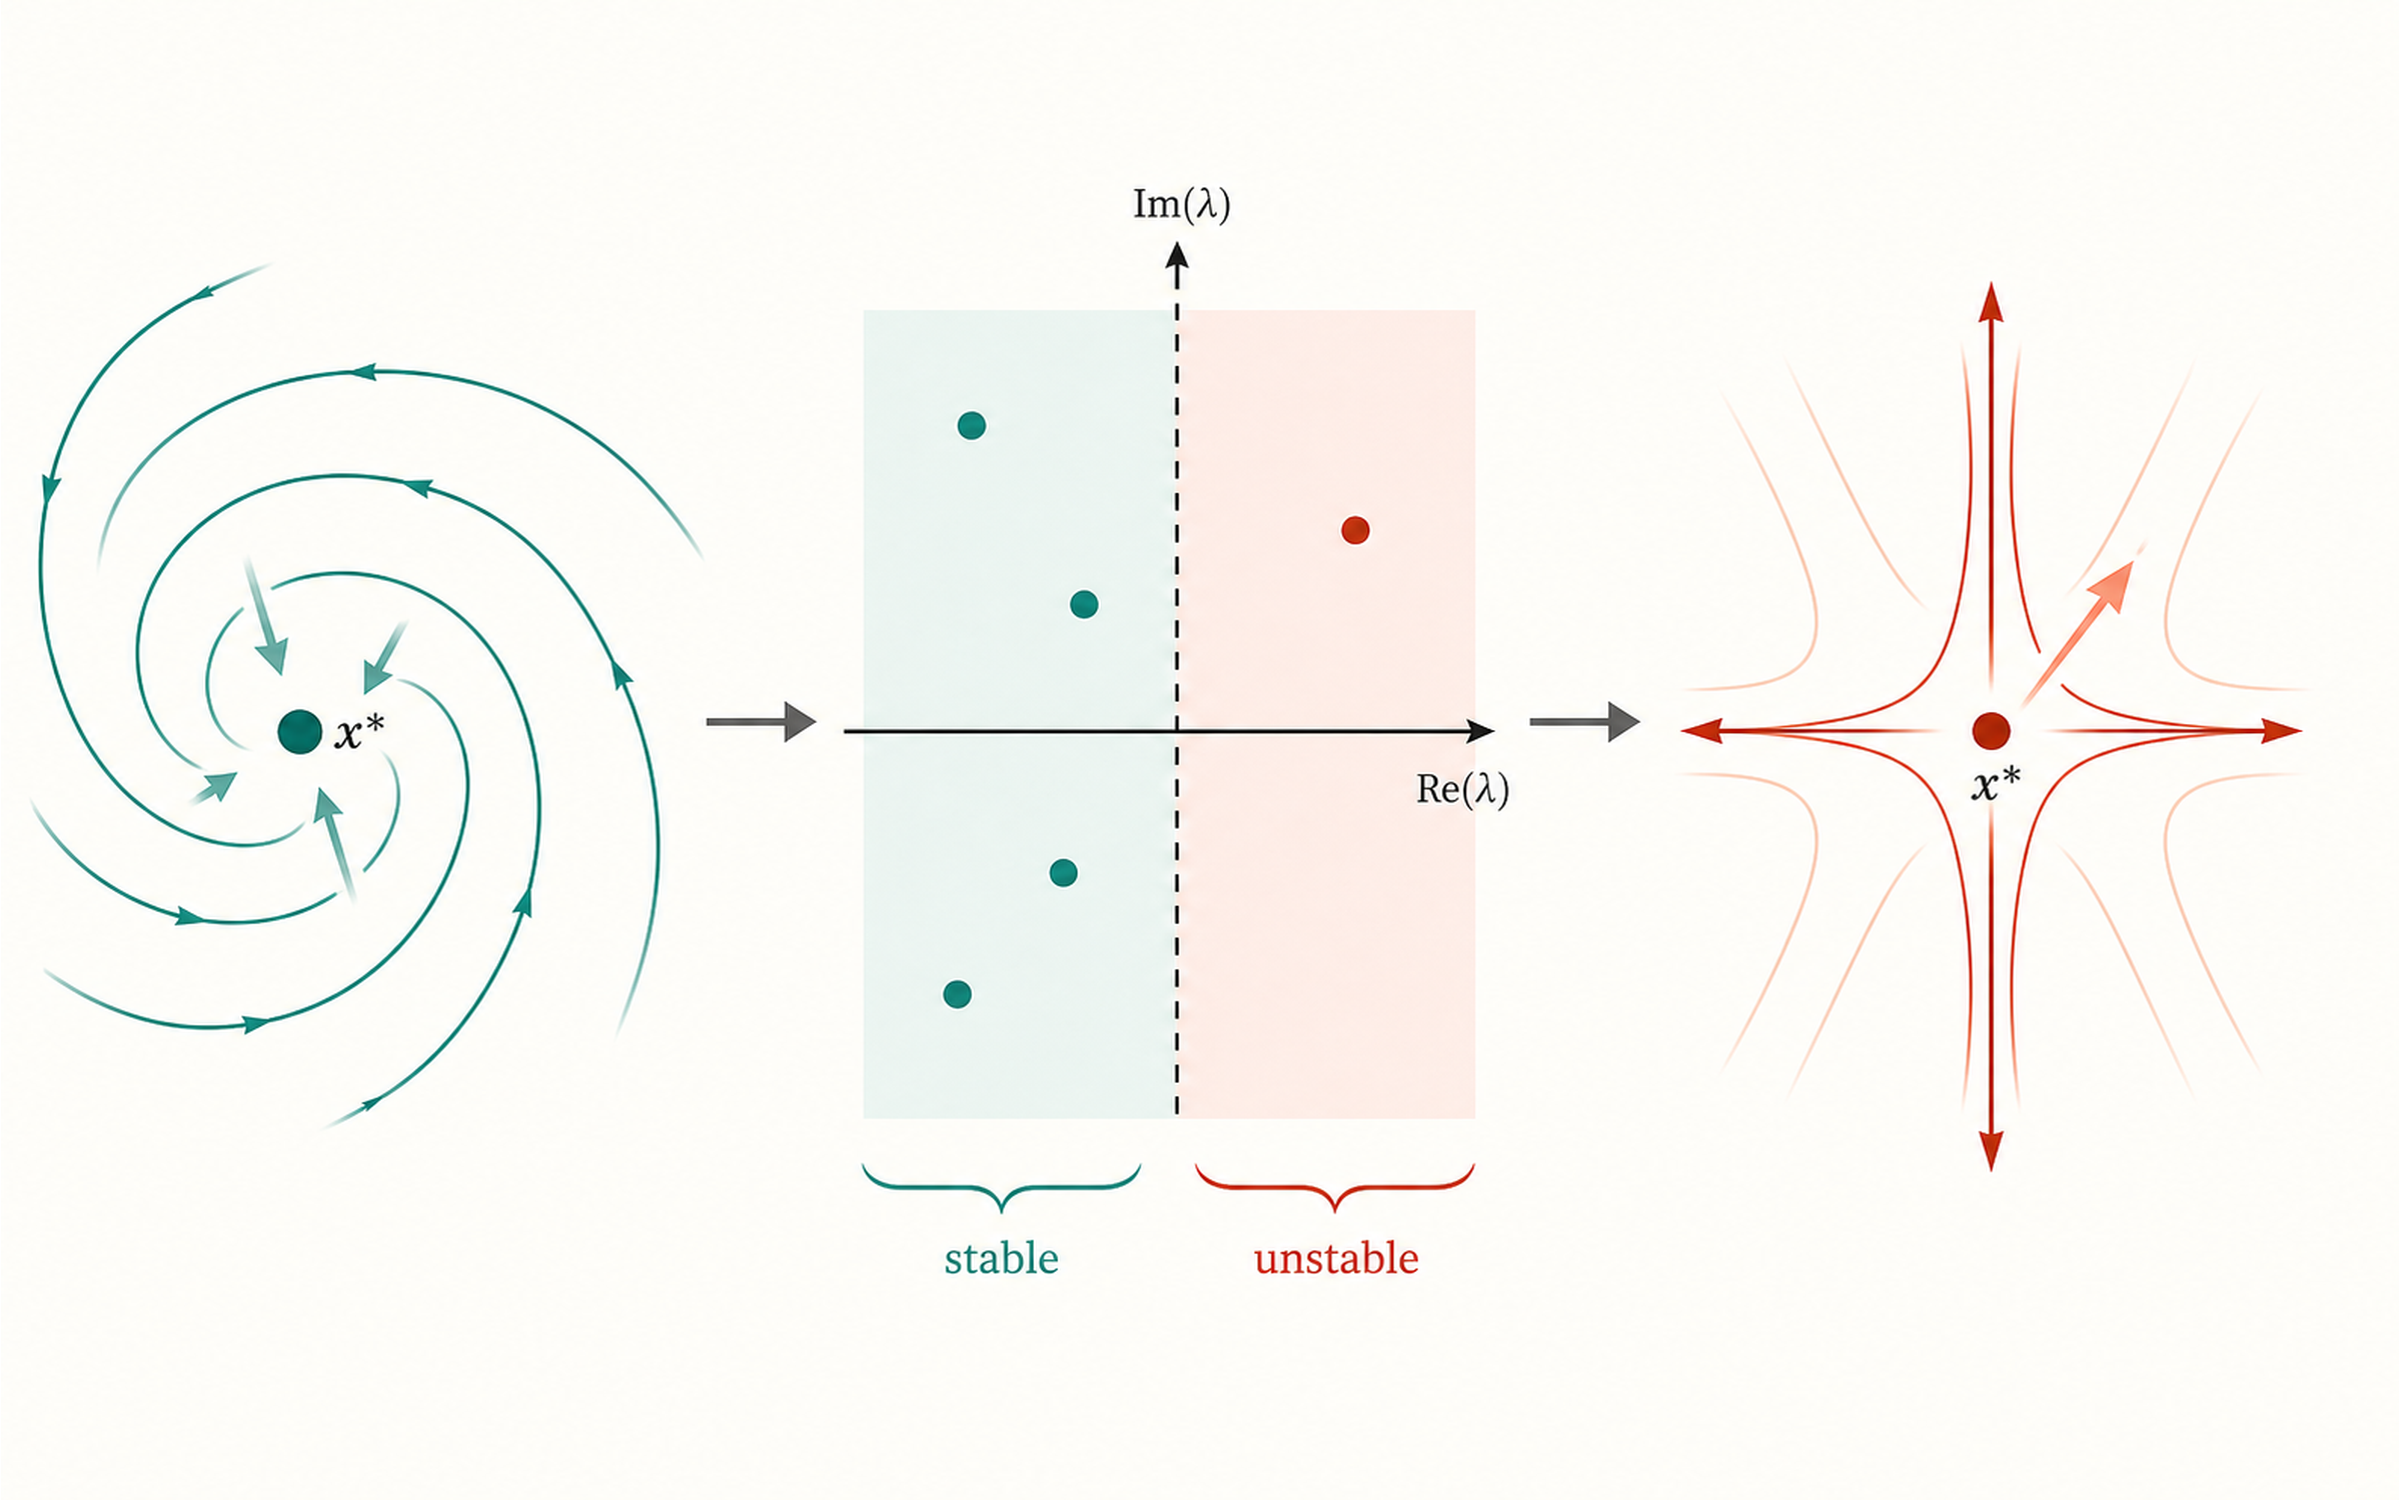
\includegraphics[width=\textwidth]{figures/imagegen/ch01-jacobian-eigenvalues-img.png}
\caption{Local stability is encoded by the Jacobian spectrum. If all eigenvalues of $J(x^\ast)$ have negative real part, infinitesimal perturbations decay toward the fixed point. If any eigenvalue has positive real part, at least one perturbation direction grows. This is the local version of the perturbation-recovery test used later to distinguish stable attractors from chaotic mesoscale dynamics.}
\label{fig:ch01-jacobian-eigenvalues}
\end{figure}

% ============================================================
\section{Attractors and Basins}
\label{sec:attractors-basins}
% ============================================================

Fixed points are only one kind of long-term behavior. An \emph{attractor} is a set $\mathcal{A}$ in state space that satisfies two properties:

\begin{enumerate}
  \item If a trajectory starts in $\mathcal{A}$, it remains in $\mathcal{A}$.
  \item Trajectories starting from a surrounding set of initial conditions approach $\mathcal{A}$ as $t$ increases.
\end{enumerate}

The surrounding set is the \emph{basin of attraction}. A stable fixed point, a stable limit cycle, and a chaotic attractor are all attractors, but they have different internal dynamics. A stable fixed point has no motion once reached. A limit cycle repeats. A chaotic attractor keeps moving irregularly while remaining bounded.

For clustered networks, the attractor language gives a clean interpretation of an ``active-cluster state.'' Suppose a subset $S\subseteq\{1,\ldots,Q\}$ of clusters has high activity and the remaining clusters are low. If the deterministic mesoscopic dynamics return to that same activity pattern after small perturbations, then the pattern behaves like an attractor or at least like a long-lived metastable state.

\begin{figure}[h]
\centering
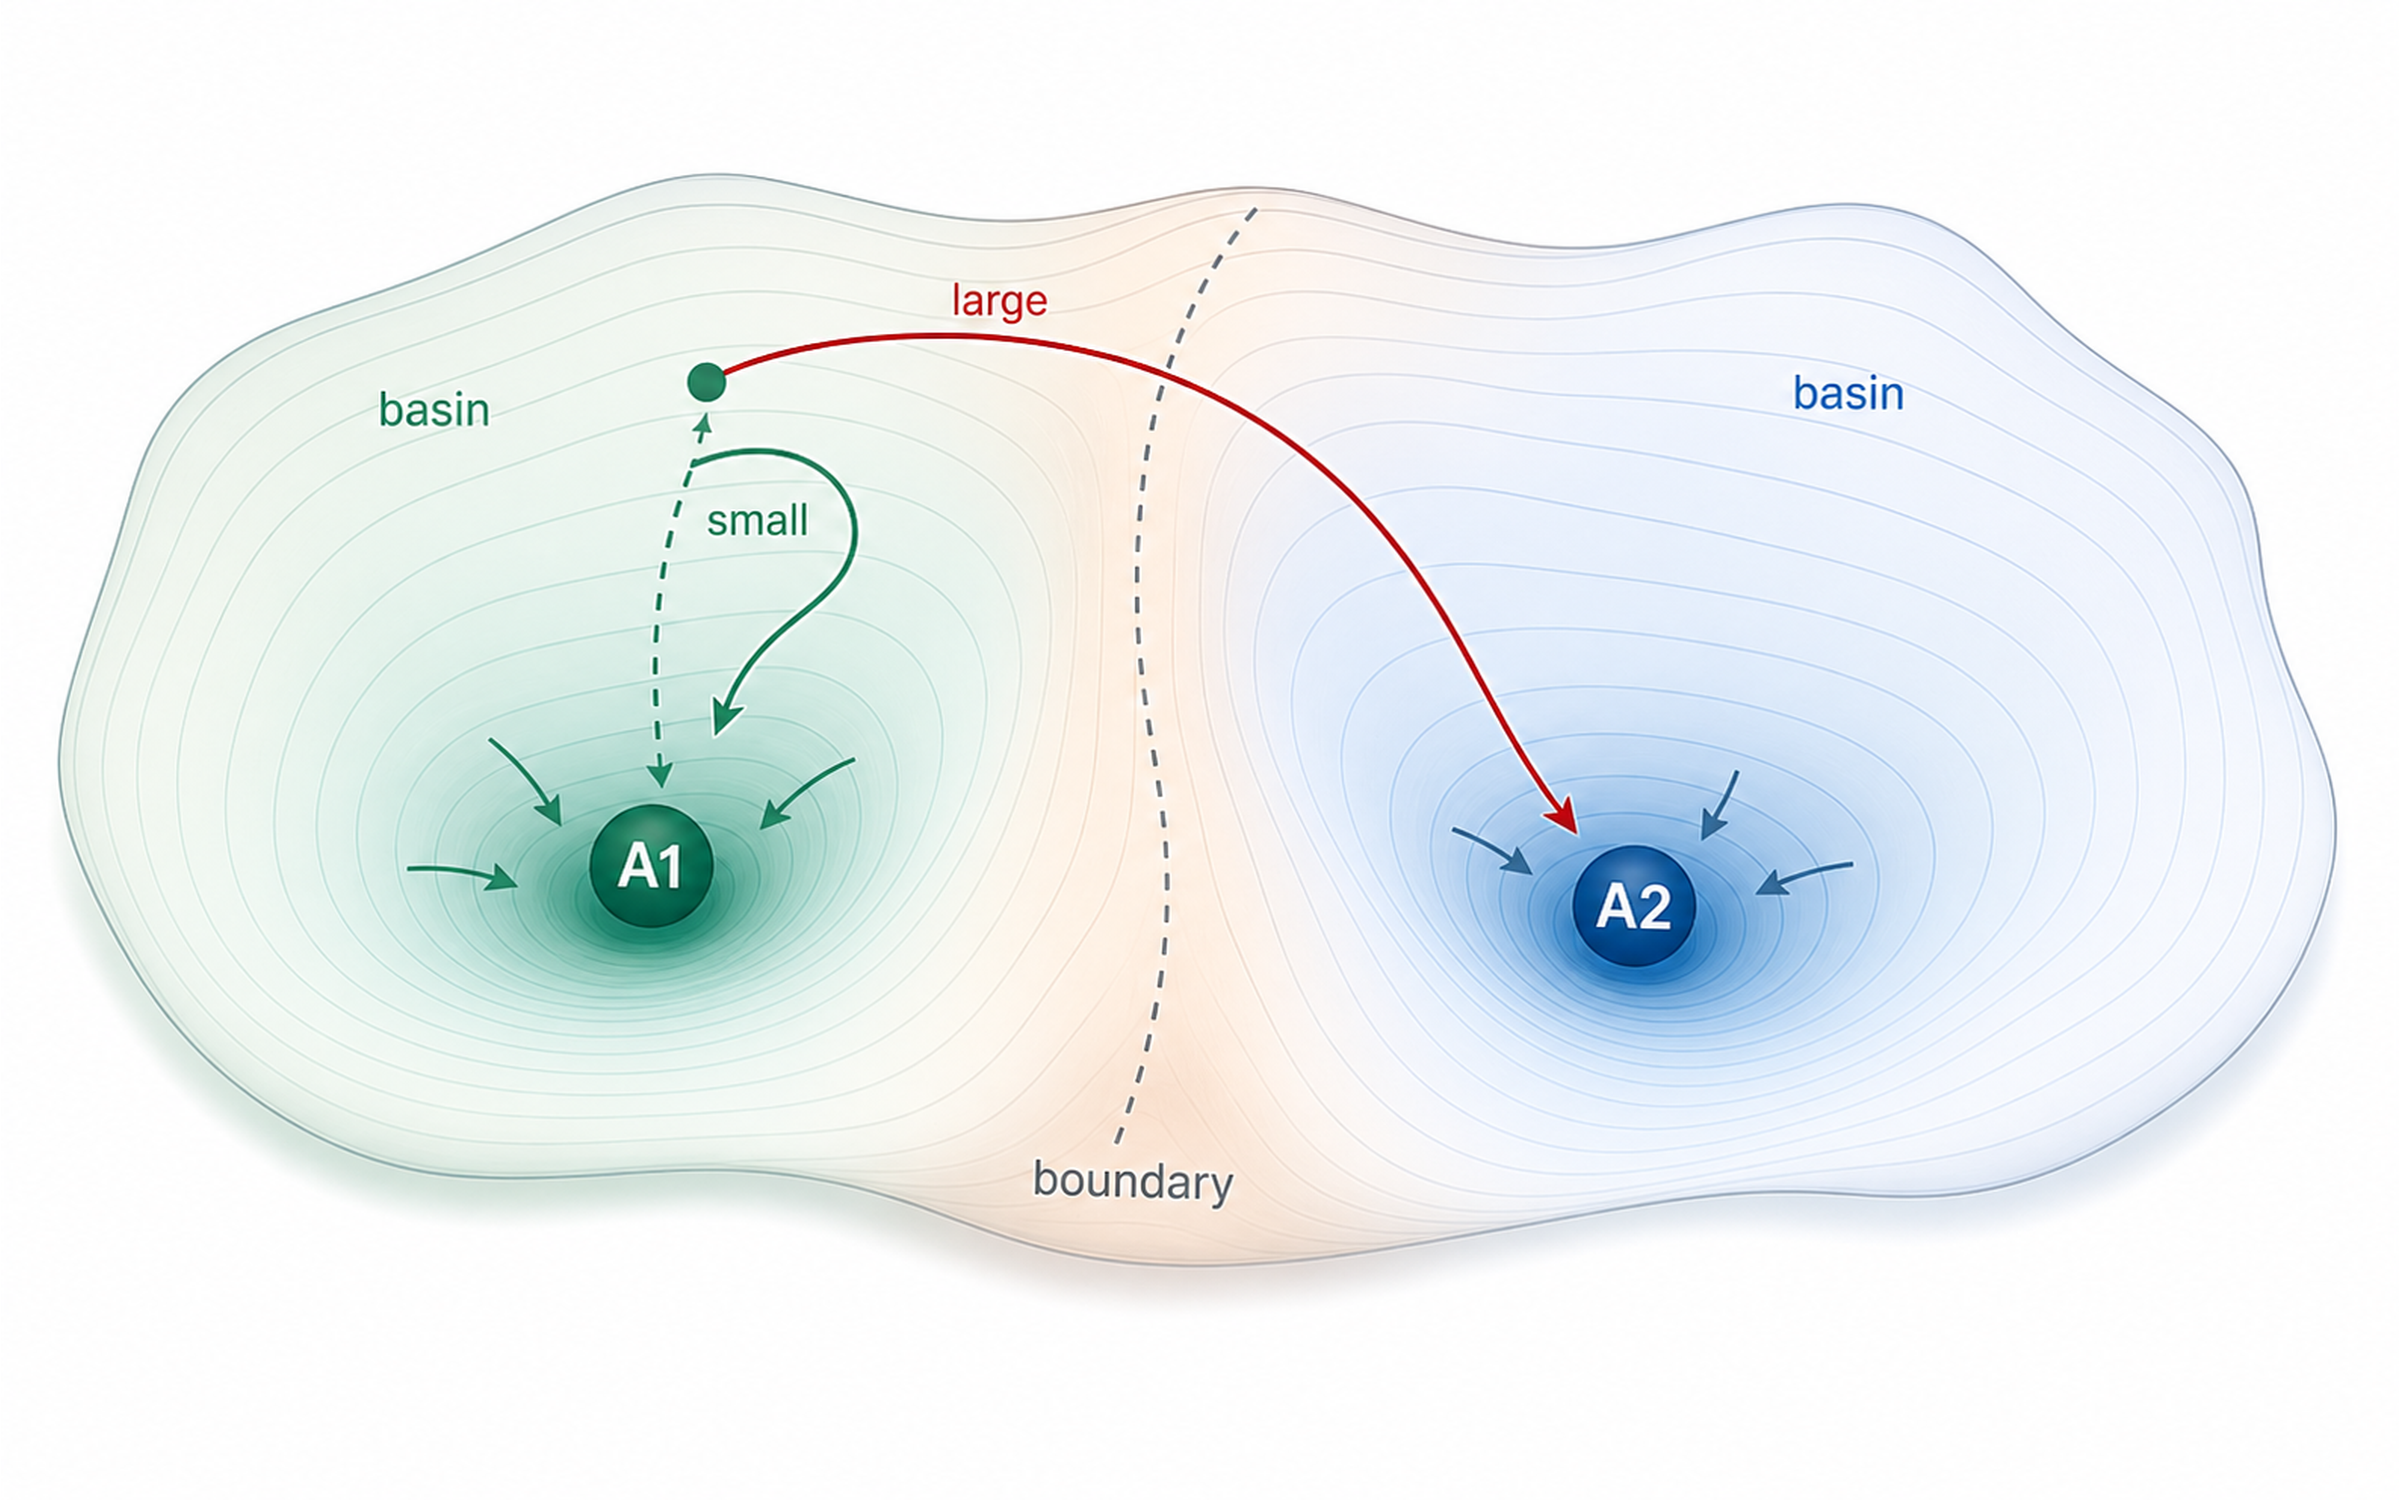
\includegraphics[width=\textwidth]{figures/imagegen/ch01-attractor-landscape-img.png}
\caption{A state-space picture of multistability. Each basin contains initial conditions that flow to the same attractor. Small perturbations inside a basin decay back to the same activity pattern, while sufficiently large perturbations can cross a basin boundary and produce a switch. In finite clustered networks, random fluctuations can play the role of repeated small perturbations.}
\label{fig:ch01-attractor-landscape}
\end{figure}

The basin picture also explains why a time trace alone can be misleading. If finite-size noise repeatedly kicks the state across basin boundaries, the observed activity switches. The switching is real, but the deterministic skeleton is still multistable. By contrast, if the deterministic mesoscopic dynamics themselves have no stable fixed active-cluster state, switching can persist even when finite-size noise is removed.

% ============================================================
\section{Multistability and Metastability}
\label{sec:multistability-metastability}
% ============================================================

A system is \emph{multistable} when it has more than one attractor for the same parameter values. Which attractor is reached depends on the initial condition and on perturbations. In a clustered attractor network, different attractors can correspond to different subsets of active clusters:
%
\begin{equation}
  S = \{c_1,\ldots,c_M\}
  \quad \longleftrightarrow \quad
  \text{clusters } c_1,\ldots,c_M \text{ active}.
  \label{eq:cluster-state-as-set}
\end{equation}
%
This representation is not a new model; it is a coarse label for regions of state space.

\emph{Metastability} means that the system spends long times near such states but eventually leaves them. There are two mechanisms that later chapters must keep separate.

First, the deterministic system may be genuinely multistable, while finite-size fluctuations drive rare basin escapes. Then increasing the number of neurons per excitatory cluster, $N_E$, reduces the fluctuation size. Switches should slow down and may disappear in the large-population limit.

Second, the mesoscopic dynamics may be chaotic because of quenched inter-cluster variability. Then switching is not an escape from a stable basin. It is part of the deterministic macroscopic motion. Switches can persist as $N_E\to\infty$.

The perturbation test follows immediately from this distinction. In a stable basin, a small perturbation decays on a local relaxation timescale set by eigenvalues of the Jacobian. In chaotic mesoscale dynamics, an arbitrarily small perturbation along an unstable direction grows exponentially for a finite time. That growth is measured by Lyapunov exponents.

% ============================================================
\section{Bifurcations}
\label{sec:bifurcations}
% ============================================================

A \emph{bifurcation} occurs when a qualitative feature of the dynamics changes as a parameter varies. In neural networks, the parameter might be external drive, E/I balance, within-cluster potentiation, or the strength of quenched inter-cluster heterogeneity.

The simplest example is a saddle-node bifurcation in one dimension:
%
\begin{equation}
  \dot{x} = \mu - x^2.
  \label{eq:saddle-node-normal-form}
\end{equation}
%
For $\mu<0$ there are no fixed points. For $\mu>0$ there are two fixed points, $x^\ast=\pm\sqrt{\mu}$. The derivative is $F'(x)=-2x$, so $+\sqrt{\mu}$ is stable and $-\sqrt{\mu}$ is unstable. At $\mu=0$, the two collide. This is a minimal model of an attractor appearing or disappearing.

In higher dimensions, common bifurcations include:

\begin{description}
  \item[Saddle-node bifurcation.] A stable and an unstable fixed point are created or annihilated.
  \item[Pitchfork-like symmetry breaking.] A symmetric state loses stability and multiple structured states appear.
  \item[Hopf bifurcation.] A fixed point loses stability to oscillatory motion when a complex-conjugate eigenvalue pair crosses the imaginary axis.
  \item[Transition to chaos.] Stable fixed points or cycles give way to a bounded but aperiodic attractor with sensitive dependence on initial conditions.
\end{description}

For clustered networks, increasing a cluster-strength parameter can create active-cluster attractors. Increasing quenched variability $\kappa$ can destabilize regular states and promote chaotic cluster-level motion. Here $\kappa$ means a fixed disorder amplitude in the inter-cluster connectivity, such as variability in $\check{J}_{ab}^{\alpha\beta}$ or in sparse Bernoulli adjacency variables $\Gamma_{ab}^{\alpha\beta}$. It is held fixed across repeated trials of the same network and is therefore distinct from finite-size spiking noise. The important point is that a phase diagram is a map of bifurcations and dynamical regimes, not merely a catalog of example traces.

% ============================================================
\section{Chaos and Lyapunov Exponents}
\label{sec:chaos-lyapunov}
% ============================================================

Chaos is deterministic irregular motion with sensitive dependence on initial conditions. The word ``deterministic'' matters: if two trajectories start from exactly the same state and evolve under the same deterministic equations, they are identical. But if their initial states differ by an arbitrarily small amount, the difference can grow exponentially before saturating at the size of the attractor.

Let $x(t)$ and $\tilde{x}(t)$ be two nearby trajectories, and define their separation
%
\begin{equation}
  \Delta(t) = \|\tilde{x}(t)-x(t)\|.
  \label{eq:trajectory-separation}
\end{equation}
%
The largest Lyapunov exponent is
%
\begin{equation}
  \lambda_{\max}
  =
  \lim_{t\to\infty}
  \frac{1}{t}
  \log\frac{\Delta(t)}{\Delta(0)}
  \label{eq:largest-lyapunov}
\end{equation}
%
when the limit exists and the initial separation is infinitesimal. If $\lambda_{\max}>0$, nearby trajectories separate exponentially on average. The associated Lyapunov time $1/\lambda_{\max}$ is the timescale over which predictive memory of the initial condition is lost.

For a stable fixed point, all perturbations decay, so the largest Lyapunov exponent is negative. For a stable limit cycle, the largest exponent is zero because perturbations along the phase direction neither grow nor decay asymptotically. For chaos, the largest exponent is positive.

\begin{figure}[t]
\centering
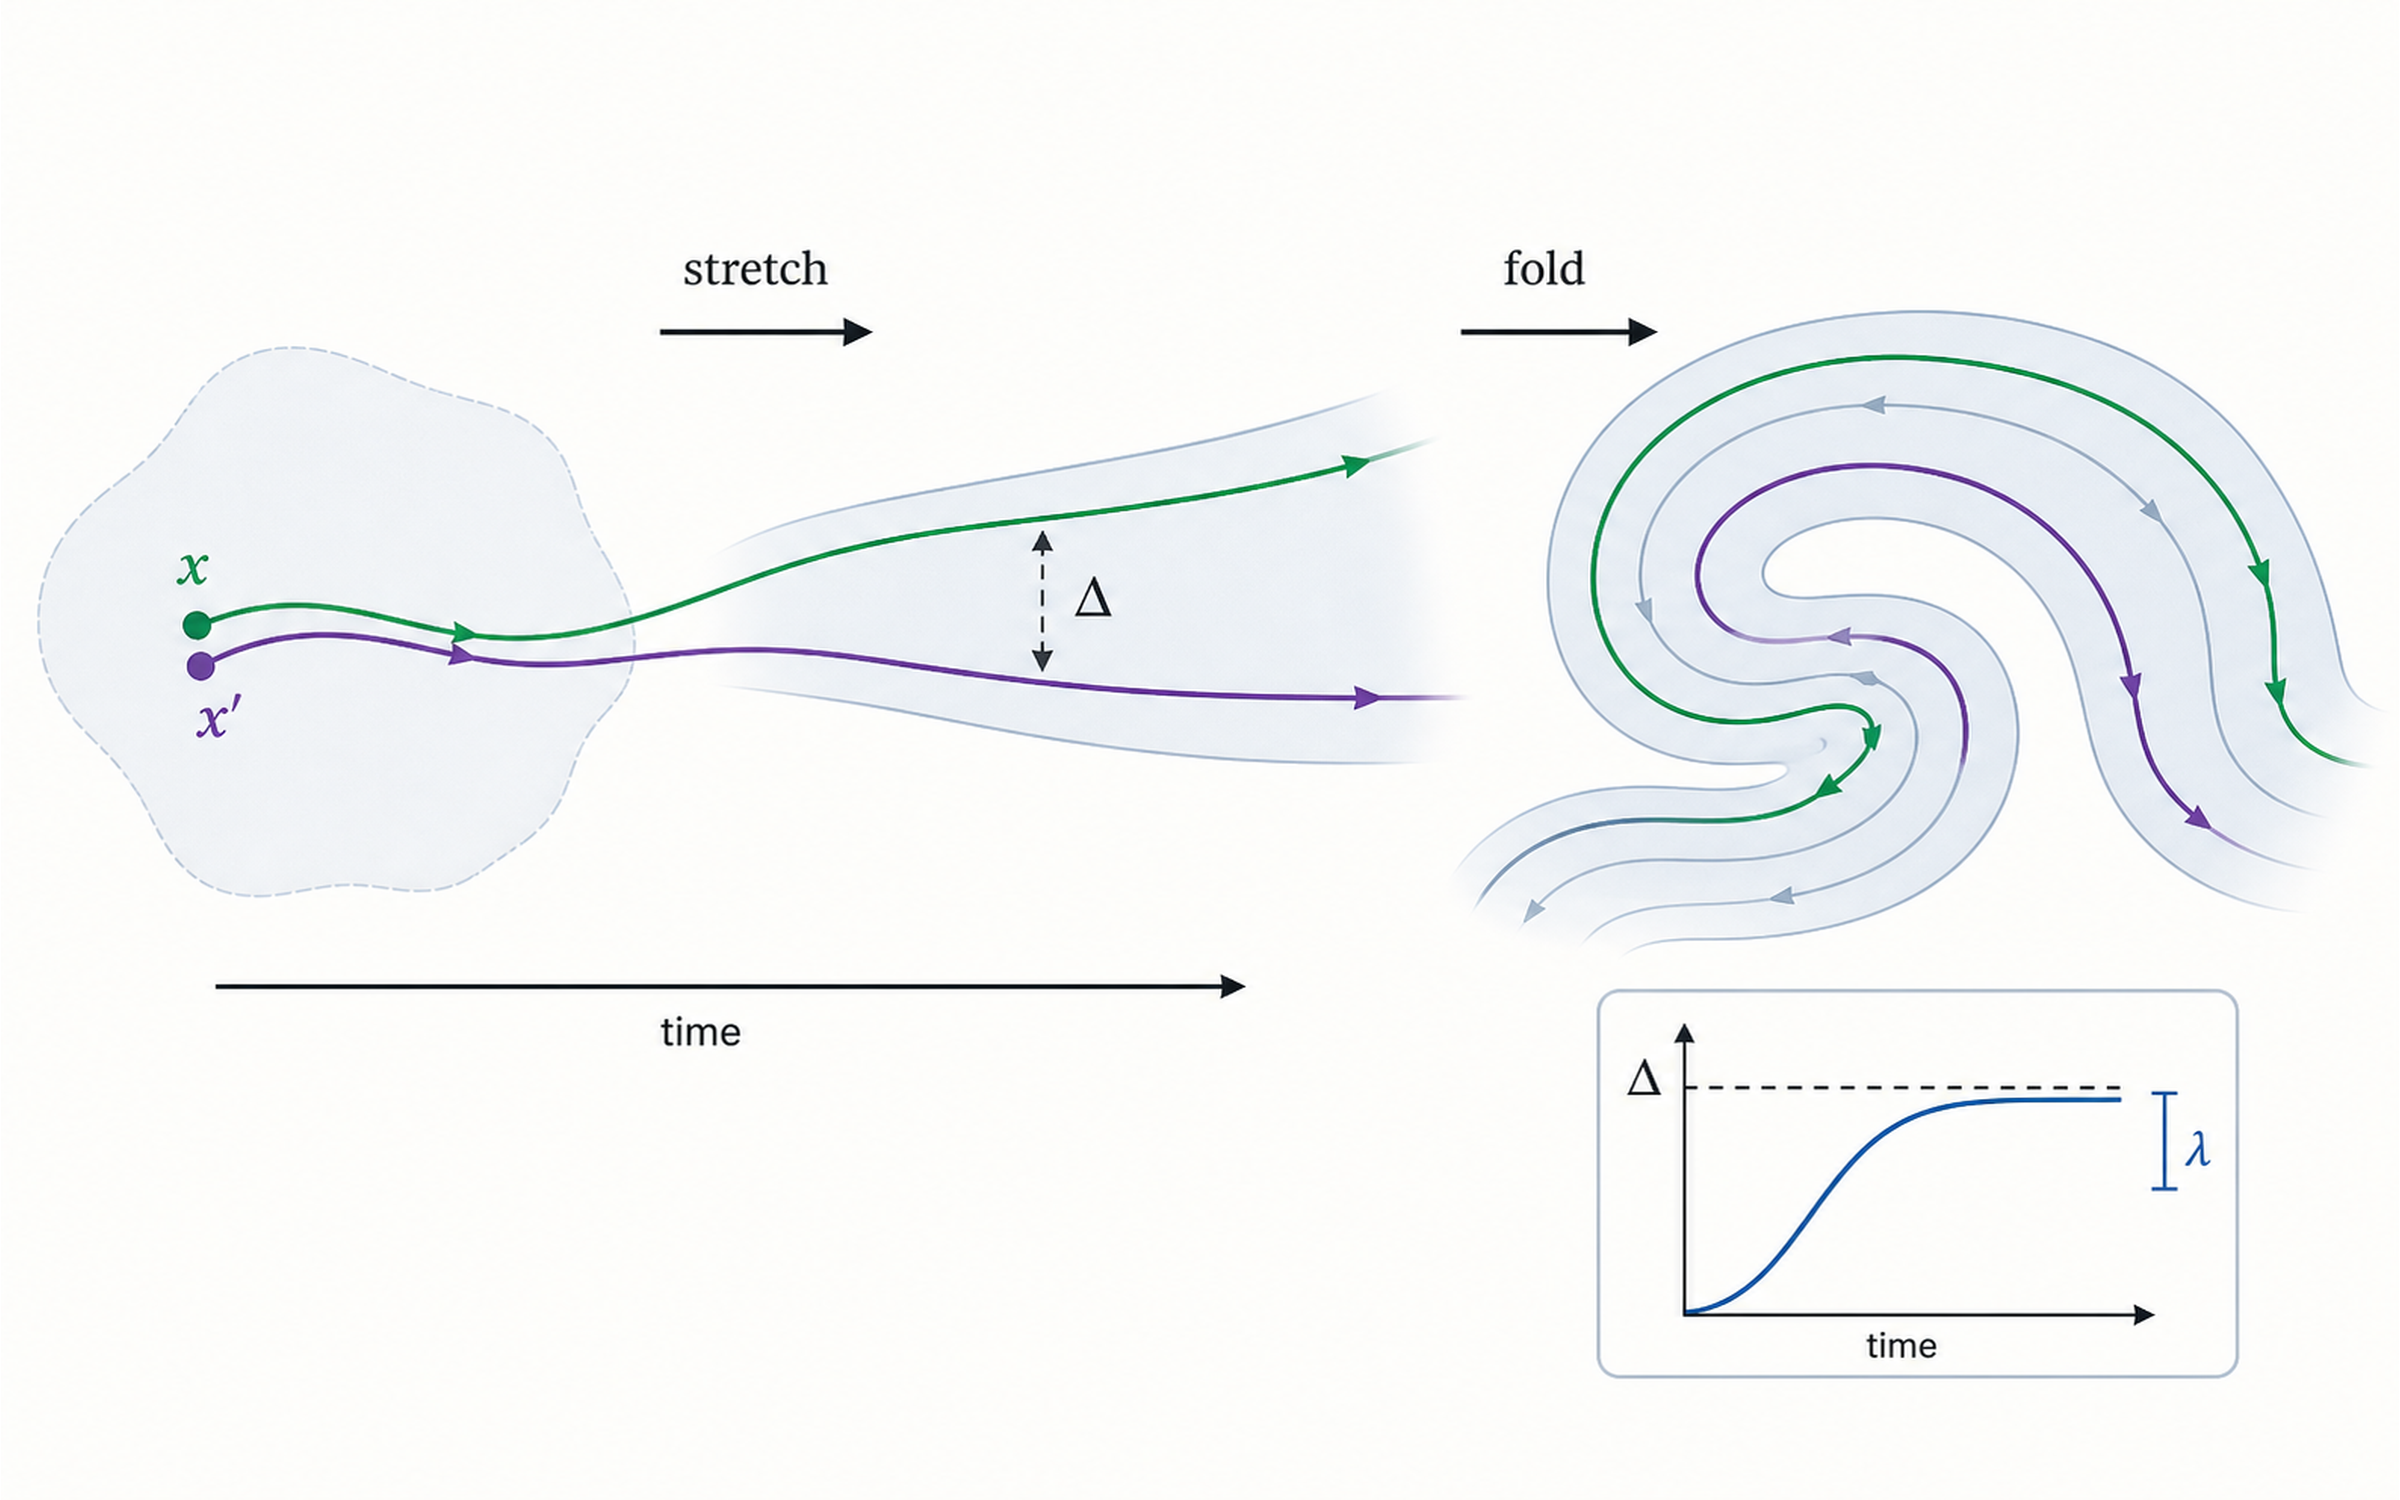
\includegraphics[width=\textwidth]{figures/imagegen/ch01-lyapunov-stretch-fold-img.png}
\caption{Lyapunov sensitivity in a bounded chaotic flow. Two trajectories begin nearly on top of each other, separate along an expanding direction, and are then folded back by the nonlinear dynamics. The separation can grow approximately like $\Delta(t)\approx \Delta(0)e^{\lambda t}$ for a finite window even though the trajectories remain confined to the attractor.}
\label{fig:ch01-lyapunov-stretch-fold}
\end{figure}

In stochastic spiking networks, Lyapunov diagnostics require care. If two runs receive independent random spike noise, their differences grow partly because the noise is different. To test deterministic sensitivity, one should compare trajectories under the same frozen disorder and, when appropriate, the same noise realization. Later chapters use this idea at the mesoscale: finite-size effects are indexed by
%
\begin{equation}
  \xi = \frac{1}{\sqrt{N_E}},
  \label{eq:xi-preview}
\end{equation}
%
whereas quenched inter-cluster variability is indexed by the fixed disorder amplitude $\kappa$. The dynamical question is what remains as $\xi\to 0$ at fixed $\kappa$.

% ============================================================
\section{The Diagnostic Logic We Will Reuse}
\label{sec:diagnostic-logic}
% ============================================================

This chapter gives the core diagnostic logic for the course:

\begin{enumerate}
  \item Identify the state variables $x(t)$ at the resolution of interest.
  \item Ask whether candidate activity patterns are fixed points, cycles, or more complicated invariant sets.
  \item Use local stability, Jacobian eigenvalues, and perturbation recovery to test whether nearby trajectories return.
  \item Use bifurcation parameters to organize regimes.
  \item Use Lyapunov exponents to decide whether deterministic mesoscopic motion has sensitive dependence on initial conditions.
\end{enumerate}

The next chapter adds the stochastic objects needed for spiking networks: spike trains, point processes, synaptic filtering, autocorrelations, and the $1/\sqrt{N_E}$ scaling of finite-size fluctuations. Those tools explain why a finite network can switch even when the deterministic state-space picture contains stable basins.

\begin{center}
\renewcommand{\arraystretch}{1.35}
\begin{tabular}{p{0.24\textwidth} p{0.34\textwidth} p{0.34\textwidth}}
\hline
\textbf{Concept} & \textbf{Mathematical test} & \textbf{Later use} \\
\hline
Stable attractor & Perturbations decay; local eigenvalues have negative real parts near a fixed point & Multistable active-cluster states \\
Basin boundary & Initial conditions on different sides approach different attractors & Noise-driven switching between metastable states \\
Bifurcation & Qualitative change as a parameter varies & Phase diagrams in cluster strength and heterogeneity \\
Chaos & Largest Lyapunov exponent positive & Mesoscopic switching that persists as finite-size noise vanishes \\
\hline
\end{tabular}
\end{center}
